\documentclass{beamer}
%
% Choose how your presentation looks.
%
% For more themes, color themes and font themes, see:
% http://deic.uab.es/~iblanes/beamer_gallery/index_by_theme.html
%
\mode<presentation>
{
  \usetheme{Madrid}      % or try Darmstadt, Madrid, Warsaw, ...
  \usecolortheme{default} % or try albatross, beaver, crane, ...
  \usefonttheme{default}  % or try serif, structurebold, ...
  \setbeamertemplate{navigation symbols}{}
  \setbeamertemplate{caption}[numbered]
} 

\usepackage[english]{babel}
\usepackage[utf8x]{inputenc}
\usepackage{hyperref}
\hypersetup{
    colorlinks = True,
    linkbordercolor = {white}
}

\title[ISU-01-06]{Processing ddRAD for population history inference}
\author{April Wright}
\institute{ISU and KU}
\date{01-06-2016}

\begin{document}

\begin{frame}
  \titlepage
\end{frame}

% Uncomment these lines for an automatically generated outline.
%\begin{frame}{Outline}
%  \tableofcontents
%\end{frame}

\section{Introduction}

\begin{frame}{Introduction}

\frametitle{ddRAD data}
\begin{itemize}
\item Reduced-representation genomic method
\end{itemize}
\end{frame}

\begin{frame}
\frametitle{ddRAD data}
\begin{itemize}
\item Reduced-representation genomic method
\item Cheap
\end{itemize}
\end{frame}

\begin{frame}
\frametitle{ddRAD data}
\begin{itemize}
\item Reduced-representation genomic method
\item Cheap
\item Lots of data returned
\end{itemize}
\end{frame}

\begin{frame}
\frametitle{ddRAD data}
\begin{itemize}
\item Reduced-representation genomic method
\item Cheap
\item Lots of data returned
\item Stable software pipelines for using these data
\end{itemize}
\end{frame}

\begin{frame}
\frametitle{A Quick Note}
Slides that contain ddRAD specific info will be noted. Some steps can be used with multiple data sources.
\end{frame}

\begin{frame}
\frametitle{Our Study}
\begin{block}{The Edwards Plateau}
% Your image included here
\begin{figure}
    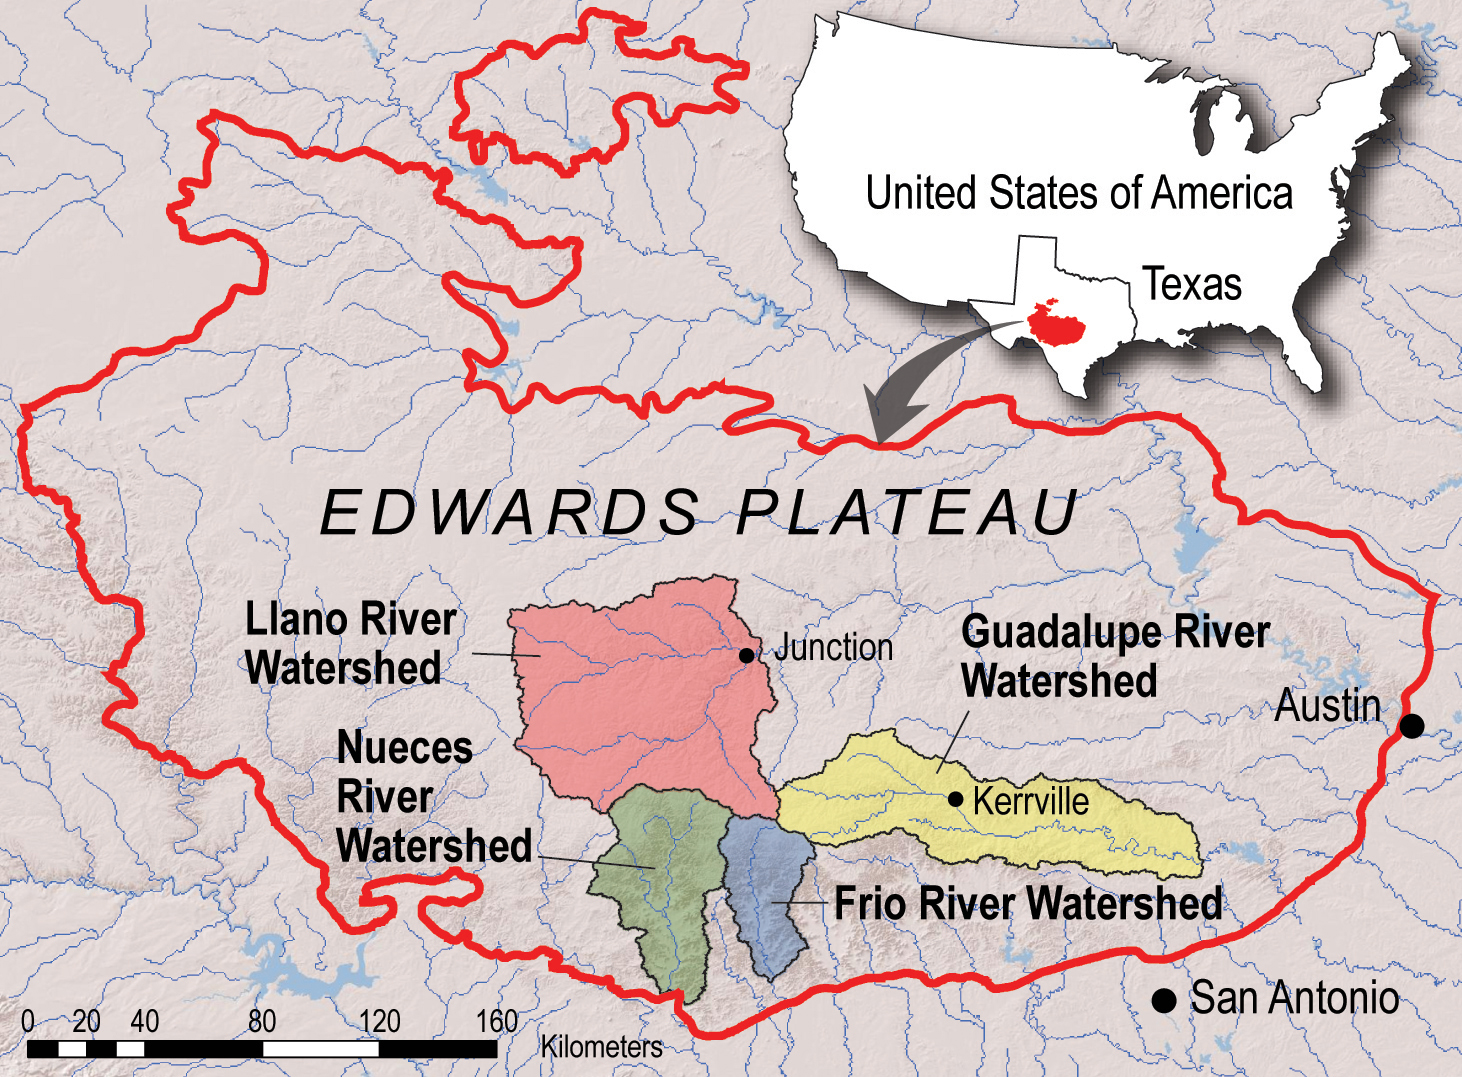
\includegraphics[scale=0.15]{pr_2010-06_map_hi-res.jpg}
    \caption{Image: AGU}
    \end{figure}
    \end{block}
\end{frame}

\begin{frame}
\frametitle{Our Study}
\begin{figure}
    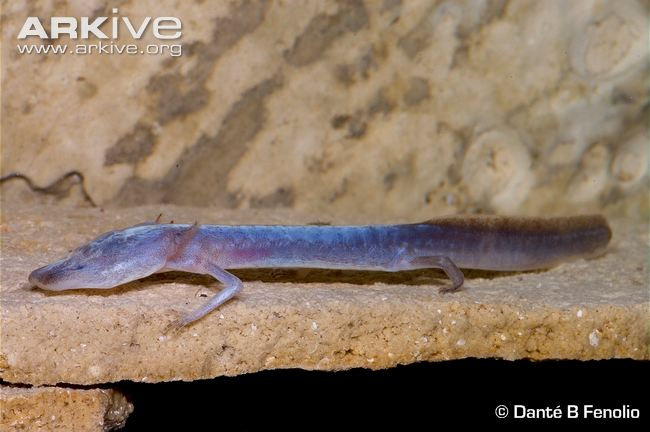
\includegraphics[scale=0.65]{Long-shot-of-Austin-blind-salamander.jpg}
    \end{figure}
\end{frame}

\begin{frame}
\frametitle{Our Study}
13 putative species of \textit{Eurycea}
\end{frame}

\begin{frame}
\frametitle{Our Study}
13 putative species of \textit{Eurycea} \\
All of which are fairly threatened by development
\end{frame}

\begin{frame}
\frametitle{Phylogenetics}
\begin{itemize}
\item Maximum likelihood
\item Statistically consistent
\end{itemize}
\end{frame}

\begin{frame}
\frametitle{Phylogenetics}
\begin{itemize}
\item Maximum likelihood
\item Statistically consistent
\item Superimposed changes
\end{itemize}
\end{frame}

\begin{frame}
\frametitle{Phylogenetics}
\begin{itemize}
\item Maximum likelihood
\item Statistically consistent
\item Superimposed changes
\item Model-based 
\end{itemize}
\end{frame}

\begin{frame}
\frametitle{Phylogenetics}
\begin{itemize}
\item \textbf{Problems}
\end{itemize}
\end{frame}

\begin{frame}
\frametitle{Phylogenetics}
\begin{itemize}
\item \textbf{Problems}
\item Missing data
\end{itemize}
\end{frame}

\begin{frame}
\frametitle{Phylogenetics}
\begin{itemize}
\item \textbf{Problems}
\item \textbf{Biased} Missing data
\end{itemize}
\end{frame}

\begin{frame}
\frametitle{Phylogenetics}
\begin{itemize}
\item Missing data concentrated in specific individuals
\end{itemize}
\end{frame}

\begin{frame}
\frametitle{Phylogenetics}
\begin{itemize}
\item Missing data concentrated in specific individuals
\item Missing data concentrated in certain sites in the alignment
\end{itemize}
\end{frame}

\begin{frame}
\frametitle{Phylogenetics}
Today, we'll be visualizing our data at every step to try and minimize a bias in which individuals have missing data
\end{frame}

\begin{frame}
\frametitle{Phylogenetics}
We'll also look at ways to make sure we aren't overly-conservative in our choosing of SNPs (i.e., biasing our collection towards sites that exhibit little change)
\end{frame}

\begin{frame}
\frametitle{The Demultiplex}
One of the things that makes RADseq, and especially ddRADseq, so cheap is the pooling of samples
\end{frame}

\begin{frame}
\frametitle{The Demultiplex}
One of the things that makes RADseq, and especially ddRADseq, so cheap is the pooling of samples \\
The way we recover individual samples is via demultiplexing
\end{frame}

\begin{frame}
\frametitle{The Demultiplex}
This allows for the cost-saving properties of batching, without the cost-increasing properties of synthesizing oligonucleotides. 
\end{frame}

\begin{frame}
\frametitle{The Demultiplex}
We'll be using STACKS for this step
\end{frame}

\begin{frame}
\frametitle{The Demultiplex}
We'll be using STACKS for this step
The STACKS step for this is called \href{http://catchenlab.life.illinois.edu/stacks/comp/process_radtags.php}{Process RAD Tags} 
\end{frame}

\begin{frame}
\frametitle{The Demultiplex}
\begin{itemize}
\item \noindent \textbf{Key Parameters}
\end{itemize}
\end{frame}

\begin{frame}
\frametitle{The Demultiplex}
\noindent \textbf{Key Parameters}
\begin{itemize}
\item -b: A path to your barcodes file
\end{itemize}
\end{frame}

\begin{frame}
\frametitle{The Demultiplex}
\noindent \textbf{Key Parameters}
\begin{itemize}
\item -b: A path to your barcodes file
\item -o: A path to where you want to put your output
\end{itemize}
\end{frame}

\begin{frame}
\frametitle{The Demultiplex}
\noindent \textbf{Key Parameters}
\begin{itemize}
\item -b: A path to your barcodes file
\item -o: A path to where you want to put your output
\item -q: Discard low-quality reads
\item -D: capture the discarded reads in a file
\end{itemize}
\end{frame}

\begin{frame}
\frametitle{The Demultiplex}
\noindent \textbf{Parameters You Will Get From the Sequencing Center}
\begin{itemize}
\item --inline/index: How are the combinatorial barcodes stored in the data?
\item Restriction enzymes
\item -f: Name of the file. Either this will be the file you downloaded, or something you renamed
\end{itemize}
\end{frame}

\begin{frame}
\frametitle{The Demultiplex}
Putting it all together: processrad.sh
\end{frame}

\begin{frame}
\frametitle{The Demultiplex}
Let's look at the output
\end{frame}

\begin{frame}
\frametitle{The Demultiplex}
Let's look at the output
\begin{itemize}
\item FASTQ files
\end{itemize}
\end{frame}

\begin{frame}
\frametitle{The Demultiplex}
Let's look at the output
\begin{itemize}
\item FASTQ files
\item Reads, grouped by individual
\end{itemize}
\end{frame}

\begin{frame}
\frametitle{The Demultiplex}
Let's look at the output
\begin{itemize}
\item FASTQ files
\item Reads, grouped by individual
\item We haven't done any SNP calling. This is just the step that gets our data ready to do that
\end{itemize}
\end{frame}

\begin{frame}
\frametitle{Initial Identification of SNPs}
For this step, we will use \href{http://catchenlab.life.illinois.edu/stacks/comp/ustacks.php}{ustacks}
\end{frame}

\begin{frame}
\frametitle{Initial Identification of SNPs}
Each RAD tag has usually been sequenced multiply per-individual
\end{frame}

\begin{frame}
\frametitle{Initial Identification of SNPs}
Each RAD tag has usually been sequenced multiply per-individual \\
This allows us to sort tags into "stacks" of identical and unique reads
\end{frame}

\begin{frame}
\frametitle{Initial Identification of SNPs}
Each RAD tag has usually been sequenced multiply per-individual \\
This allows us to sort tags into "stacks" of identical and unique reads
From these sets of identical and unique reads, we do a first pass at identifying SNPs.
\end{frame}

\begin{frame}
\frametitle{Initial Identification of SNPs}
\textbf{Key Parameters}
\begin{itemize}
\item -m: Minimum depth of coverage
\item -M: Maximum mismatches allowed between reads in a stack
\end{itemize}
\end{frame}

\begin{frame}
\frametitle{Initial Identification of SNPs}
\textbf{Other Parameters}
\begin{itemize}
\item -i: ID for this sample
\item -f: filename
\end{itemize}
\end{frame}

\begin{frame}
\frametitle{Exercise}
\textbf{Try it}
\begin{itemize}
\item Script ustacks.sh
\item Choose a different value for -m
\end{itemize}
\end{frame}


\begin{frame}
\frametitle{Exercise}
So now we have output
\end{frame}

\begin{frame}
\frametitle{Exercise}
I've included a script, calculateMissing.sh, and another, plotMissing.py
\end{frame}

\begin{frame}
\frametitle{Exercise}
One of the issues we discussed was biased missing data
\end{frame}

\begin{frame}
\frametitle{Catalog Building}
Once we have our within-individual stacks, we build a catalog of loci across individual catalogs
\end{frame}

\begin{frame}
\frametitle{Catalog Building}
\textbf{Key Parameters}
\begin{itemize}
\item -m: Maintain tags that match more than one RAD tag
\item -n: number of mismatches to allow between a putative tag, and a tag in the catalog
\end{itemize}
\end{frame}

\begin{frame}
\frametitle{Catalog Building}
\textbf{Exercise}
\begin{itemize}
\item cstacks.sh
\item Choose a different value for -n
\end{itemize}
\end{frame}

\begin{frame}
\frametitle{Catalog Building}
\textbf{Exercise}
\begin{itemize}
\item Run the two error-checking scripts
\end{itemize}
\end{frame}

\begin{frame}
\frametitle{Check Individuals Against Catalog}
We use sstacks for this
\end{frame}

\begin{frame}
\frametitle{Outputting Data for Phylogenetics}
We use populations for this. 
\end{frame}

\begin{frame}
\frametitle{Outputting Data for Phylogenetics}
A new file is needed, here: \textbf{the population map}
\end{frame}

\begin{frame}
\frametitle{Outputting Data for Phylogenetics}
\textbf{Key Parameters}
\begin{itemize}
\item -r: Percentage of individuals that must have a locus to output it
\item -m: Minimum stack depth at a locus
\end{itemize}
\end{frame}


\begin{frame}
\frametitle{Exercise}
Run the populations script. 
\end{frame}

\begin{frame}
\frametitle{Exercise}
Looking at this output is easy.
\end{frame}

\begin{frame}
\frametitle{Lastly, let's build the tree}
Run the tree building script like so:

treebuild.sh file.phylip
Email your tree to me, titled with your group number
\end{frame}


\vskip 1cm
\begin{frame}
\begin{block}{Examples}
Some examples of commonly used commands and features are included, to help you get started.
\end{block}
\end{frame}

\section{Some \LaTeX{} Examples}

\subsection{Tables and Figures}

\begin{frame}{Tables and Figures}

\begin{itemize}
\item Use \texttt{tabular} for basic tables --- see Table~\ref{tab:widgets}, for example.
\item You can upload a figure (JPEG, PNG or PDF) using the files menu. 
\item To include it in your document, use the \texttt{includegraphics} command (see the comment below in the source code).
\end{itemize}

% Commands to include a figure:
%\begin{figure}
%\includegraphics[width=\textwidth]{your-figure's-file-name}
%\caption{\label{fig:your-figure}Caption goes here.}
%\end{figure}

\begin{table}
\centering
\begin{tabular}{l|r}
Item & Quantity \\\hline
Widgets & 42 \\
Gadgets & 13
\end{tabular}
\caption{\label{tab:widgets}An example table.}
\end{table}

\end{frame}

\subsection{Mathematics}

\begin{frame}{Readable Mathematics}

Let $X_1, X_2, \ldots, X_n$ be a sequence of independent and identically distributed random variables with $\text{E}[X_i] = \mu$ and $\text{Var}[X_i] = \sigma^2 < \infty$, and let
$$S_n = \frac{X_1 + X_2 + \cdots + X_n}{n}
      = \frac{1}{n}\sum_{i}^{n} X_i$$
denote their mean. Then as $n$ approaches infinity, the random variables $\sqrt{n}(S_n - \mu)$ converge in distribution to a normal $\mathcal{N}(0, \sigma^2)$.

\end{frame}

\end{document}
